% answers.tex —— 1995 年·全国卷·理科 · 参考答案与详细解析片段
% 由 tools/generate_projects.py 依来源总账自 1995/1995_数学真题_全国理_试题.md + 1995/1995_数学真题_全国理_解析正文.md + 1995/1995_数学真题_全国理_答案要点.md 生成，勿手改（改源 MD 后重跑）


\begin{answer}
\gksolhead{1}{}

\textbf{题目}：

已知 $I$ 为全集，集合 $M,N\subseteq I$，若 $M\cap N=N$，则\mbox{（　　）}。

（A）$\overline{M}\supseteq\overline{N}$　　（B）$M\subseteq\overline{N}$　　（C）$\overline{M}\subseteq\overline{N}$　　（D）$M\supseteq\overline{N}$

\Needspace{4\baselineskip}
\textbf{解析}

由 $M\cap N=N$ 得 $N\subseteq M$。集合的包含关系在取补集时反向，故 $\overline{M}\subseteq\overline{N}$。这正是（C）。

\textbf{验算：} 取 $I=\{1,2,3,4\}$，$M=\{1,2,3\}$，$N=\{1,2\}$，则 $M\cap N=N$；$\overline{M}=\{4\}\subseteq\overline{N}=\{3,4\}$ 成立。逐项排除：$M\subseteq\overline{N}$ 假（$2\in M$ 而 $2\notin\overline{N}$）；$M\supseteq\overline{N}$ 假（$4\notin M$）；$\overline{M}\supseteq\overline{N}$ 假（$3\in\overline{N}$ 而 $3\notin\overline{M}$）。

\gkanswer{答案：C。}

\par\medskip

\end{answer}
\begin{answer}
\gksolhead{2}{}

\textbf{题目}：

函数 $y=-\dfrac{1}{x+1}$ 的图象是\mbox{（　　）}。
\nopagebreak[4]
\begin{center}% 固定来源PDF印刷页51第2题四个图象选项的矢量示意重绘。
% 渐近线位置、分支象限及选项标签忠于原页；比例仅作示意。
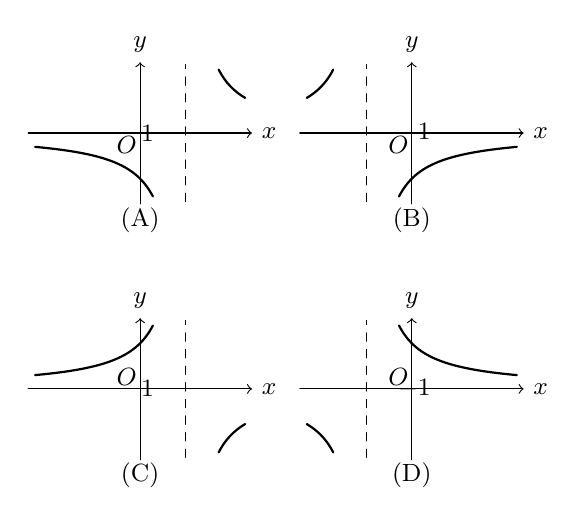
\begin{tikzpicture}[x=.58cm,y=.58cm,font=\small,line cap=round,line join=round]
  % (A) y=1/(x-1)
  \begin{scope}
    \draw[->] (-2.45,0)--(2.45,0) node[right] {$x$};
    \draw[->] (0,-1.55)--(0,1.55) node[above] {$y$};
    \draw[dashed] (1,-1.5)--(1,1.5);
    \draw[thick,domain=-2.3:.28,samples=60,variable=\x] plot (\x,{1/(\x-1)});
    \draw[thick,domain=1.72:2.3,samples=60,variable=\x] plot (\x,{1/(\x-1)});
    \node[left=8pt] at (1,0) {$1$};
    \node[below left,inner sep=1pt] at (0,0) {$O$};
    \node at (0,-1.9) {(A)};
  \end{scope}

  % (B) y=-1/(x+1), the graph of the stated function.
  \begin{scope}[xshift=3.45cm]
    \draw[->] (-2.45,0)--(2.45,0) node[right] {$x$};
    \draw[->] (0,-1.55)--(0,1.55) node[above] {$y$};
    \draw[dashed] (-1,-1.5)--(-1,1.5);
    \draw[thick,domain=-2.3:-1.72,samples=60,variable=\x] plot (\x,{-1/(\x+1)});
    \draw[thick,domain=-.28:2.3,samples=60,variable=\x] plot (\x,{-1/(\x+1)});
    \node[right=8pt] at (-1,0) {$-1$};
    \node[below left,inner sep=1pt] at (0,0) {$O$};
    \node at (0,-1.9) {(B)};
  \end{scope}

  % (C) y=-1/(x-1)
  \begin{scope}[yshift=-3.25cm]
    \draw[->] (-2.45,0)--(2.45,0) node[right] {$x$};
    \draw[->] (0,-1.55)--(0,1.55) node[above] {$y$};
    \draw[dashed] (1,-1.5)--(1,1.5);
    \draw[thick,domain=-2.3:.28,samples=60,variable=\x] plot (\x,{-1/(\x-1)});
    \draw[thick,domain=1.72:2.3,samples=60,variable=\x] plot (\x,{-1/(\x-1)});
    \node[left=8pt] at (1,0) {$1$};
    \node[above left,inner sep=1pt] at (0,0) {$O$};
    \node at (0,-1.9) {(C)};
  \end{scope}

  % (D) y=1/(x+1)
  \begin{scope}[xshift=3.45cm,yshift=-3.25cm]
    \draw[->] (-2.45,0)--(2.45,0) node[right] {$x$};
    \draw[->] (0,-1.55)--(0,1.55) node[above] {$y$};
    \draw[dashed] (-1,-1.5)--(-1,1.5);
    \draw[thick,domain=-2.3:-1.72,samples=60,variable=\x] plot (\x,{1/(\x+1)});
    \draw[thick,domain=-.28:2.3,samples=60,variable=\x] plot (\x,{1/(\x+1)});
    \node[right=8pt] at (-1,0) {$-1$};
    \node[above left,inner sep=1pt] at (0,0) {$O$};
    \node at (0,-1.9) {(D)};
  \end{scope}
\end{tikzpicture}
\end{center}
\nopagebreak[4]
\Needspace{4\baselineskip}
\textbf{解析}

$y=-\dfrac{1}{x+1}$ 的定义域为 $x\ne-1$，竖直渐近线 $x=-1$，水平渐近线 $y=0$。当 $x\to-1^{+}$ 时 $y\to-\infty$，当 $x\to-1^{-}$ 时 $y\to+\infty$；当 $x\to+\infty$ 时 $y\to0^{-}$，当 $x\to-\infty$ 时 $y\to0^{+}$。即渐近线在 $-1$ 处、左支在 $x$ 轴上方、右支在 $x$ 轴下方。按示意图，只有（B）满足：渐近线标在 $-1$，左支在上、右支在下。

\textbf{验算：} 代 $x=0$：$y=-1<0$，图（B）在 $x=0$ 处（位于渐近线右侧）确实在轴下；（A）（C）渐近线在 $x=1$ 处，不符；（D）为 $y=\dfrac{1}{x+1}$，$x=0$ 时 $y=1>0$，与（B）符号相反，不符。

\gkanswer{答案：B。}

\par\medskip

\end{answer}
\begin{answer}
\gksolhead{3}{}

\textbf{题目}：

\Needspace{5\baselineskip}
函数
\nopagebreak[4]
\[
y=4\sin\left(3x+\frac\pi4\right)+3\cos\left(3x+\frac\pi4\right)
\]
的最小正周期是\mbox{（　　）}。

（A）$6\pi$　　（B）$2\pi$　　（C）$\dfrac{2\pi}{3}$　　（D）$\dfrac\pi3$

\Needspace{4\baselineskip}
\textbf{解析}

设 $u=3x+\dfrac{\pi}{4}$，则 $y=4\sin u+3\cos u=5\sin(u+\varphi)$（$\tan\varphi=\dfrac34$）。振幅 $5\ne0$，故最小正周期等于 $u$ 变化 $2\pi$ 时 $x$ 的变化量，即 $T=\dfrac{2\pi}{3}$。

\textbf{验算：} $f(0)=4\sin\dfrac{\pi}{4}+3\cos\dfrac{\pi}{4}=\dfrac{7\sqrt2}{2}$；$f\!\left(\dfrac{2\pi}{3}\right)=4\sin\left(2\pi+\dfrac{\pi}{4}\right)+3\cos\left(2\pi+\dfrac{\pi}{4}\right)=\dfrac{7\sqrt2}{2}$ （成立）。再看 $x=\dfrac{\pi}{3}$：$u=\dfrac{5\pi}{4}$，$y=-\dfrac{7\sqrt2}{2}\ne f(0)$，故 $\dfrac{\pi}{3}$ 不是周期，$\dfrac{2\pi}{3}$ 确为最小正周期。

\gkanswer{答案：C。}

\par\medskip

\end{answer}
\begin{answer}
\gksolhead{4}{}

\textbf{题目}：

正方体的全面积是 $a^2$，它的顶点都在球面上，这个球的表面积是\mbox{（　　）}。

（A）$\dfrac{\pi a^2}{3}$　　（B）$\dfrac{\pi a^2}{2}$　　（C）$2\pi a^2$　　（D）$3\pi a^2$

\Needspace{4\baselineskip}
\textbf{解析}

设正方体棱长 $l$，全面积 $6l^2=a^2$，得 $l=\dfrac{a}{\sqrt6}$。正方体的体对角线即外接球直径：$2R=\sqrt3\,l=\dfrac{a}{\sqrt2}$，$R=\dfrac{a}{2\sqrt2}$。球的表面积 $S=4\pi R^2=4\pi\cdot\dfrac{a^2}{8}=\dfrac{\pi a^2}{2}$。

\textbf{验算（取具体值）：} 令 $a=\sqrt6$，则 $l=1$，$R=\dfrac{\sqrt3}{2}$，$S=4\pi\cdot\dfrac34=3\pi$；而 $\dfrac{\pi a^2}{2}=\dfrac{6\pi}{2}=3\pi$ （成立）。量纲：$a^2$ 为面积，与 $S$ 一致 （成立）。

\gkanswer{答案：B。}

\par\medskip

\end{answer}
\begin{answer}
\gksolhead{5}{}

\textbf{题目}：

如图，若图中的直线 $l_1,l_2,l_3$ 的斜率分别为 $k_1,k_2,k_3$，则\mbox{（　　）}。
\nopagebreak[4]
\begin{center}% 固定来源PDF印刷页51第5题斜率关系示意重绘；仅保留线条的增减趋势。
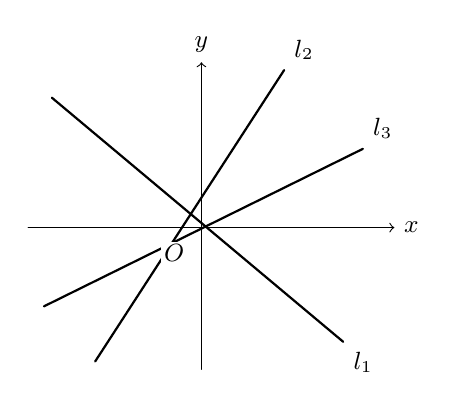
\begin{tikzpicture}[x=1cm,y=1cm,font=\small,line cap=round,line join=round]
  \draw[->] (-2.2,0)--(2.45,0) node[right] {$x$};
  \draw[->] (0,-1.8)--(0,2.1) node[above] {$y$};
  \draw[thick] (-1.9,1.65)--(1.8,-1.45) node[below right] {$l_1$};
  \draw[thick] (-1.35,-1.7)--(1.05,2.0) node[above right] {$l_2$};
  \draw[thick] (-2.0,-1.0)--(2.05,1.0) node[above right] {$l_3$};
  \node[fill=white,inner sep=1pt,below left=5pt] at (0,0) {$O$};
\end{tikzpicture}
\end{center}
\nopagebreak[4]
（A）$k_1<k_2<k_3$　　（B）$k_3<k_1<k_2$　　（C）$k_3<k_2<k_1$　　（D）$k_1<k_3<k_2$

\Needspace{4\baselineskip}
\textbf{解析}

由示意图：$l_1$ 自左向右下降，故 $k_1<0$；$l_2$、$l_3$ 均自左向右上升，故 $k_2>0,\ k_3>0$，且 $l_2$ 明显比 $l_3$ 陡，故 $0<k_3<k_2$。合起来 $k_1<k_3<k_2$，即（D）。

\textbf{验算（按图中端点估斜率）：} $l_1$ 过 $(-1.9,1.65)$、$(1.8,-1.45)$，$k_1\approx\dfrac{-3.10}{3.70}\approx-0.84$；$l_3$ 过 $(-2.0,-1.0)$、$(2.05,1.0)$，$k_3\approx\dfrac{2.0}{4.05}\approx0.49$；$l_2$ 过 $(-1.35,-1.7)$、$(1.05,2.0)$，$k_2\approx\dfrac{3.7}{2.4}\approx1.54$。故 $k_1<k_3<k_2$ （成立）。

\textbf{源疑点（说明性，非错误）：} 本题结论完全由图形给出，所用图为来源示意图的重绘，若原页图线陡缓关系与重绘不符，结论需随之复核。

\gkanswer{答案：D。}

\par\medskip

\end{answer}
\begin{answer}
\gksolhead{6}{}

\textbf{题目}：

在 $(1-x^3)(1+x)^{10}$ 的展开式中，$x^5$ 的系数是\mbox{（　　）}。

（A）$-297$　　（B）$-252$　　（C）$297$　　（D）$207$

\Needspace{4\baselineskip}
\textbf{解析}

$(1-x^3)(1+x)^{10}$ 中 $x^5$ 的系数来自两部分：$(1+x)^{10}$ 的 $x^5$ 项系数 $\mathrm C_{10}^{5}=252$，以及 $-x^3$ 乘 $(1+x)^{10}$ 的 $x^2$ 项，系数 $-\mathrm C_{10}^{2}=-45$。合计 $252-45=207$。

\textbf{验算：} 展开 $(1+x)^{10}=1+10x+45x^2+120x^3+210x^4+252x^5+\cdots$，故 $(1-x^3)(1+x)^{10}$ 的 $x^5$ 项 $=252x^5-45x^5=207x^5$ （成立）。选项中（C）$297$、（D）$207$ 同为正，只有 $207$ 与展开式一致。

\gkanswer{答案：D。}

\par\medskip

\end{answer}
\begin{answer}
\gksolhead{7}{}

\textbf{题目}：

使 $\arcsin x>\arccos x$ 成立的 $x$ 的取值范围是\mbox{（　　）}。

（A）$\left(0,\dfrac{\sqrt2}{2}\right]$　　（B）$\left(\dfrac{\sqrt2}{2},1\right]$　　（C）$\left[-1,\dfrac{\sqrt2}{2}\right)$　　（D）$[-1,0)$

\Needspace{4\baselineskip}
\textbf{解析}

\Needspace{5\baselineskip}
在 $[-1,1]$ 上恒有 $\arcsin x+\arccos x=\dfrac{\pi}{2}$。于是
\nopagebreak[4]
\[\arcsin x>\arccos x\iff \arcsin x>\frac{\pi}{4}\iff x>\sin\frac{\pi}{4}=\frac{\sqrt2}{2}.\]
结合定义域 $x\in[-1,1]$，得 $x\in\left(\dfrac{\sqrt2}{2},\,1\right]$。

\textbf{验算：} $x=1$：$\arcsin1=\dfrac{\pi}{2}>0=\arccos1$ （成立）（端点取到）；$x=\dfrac{\sqrt2}{2}$：两边都等于 $\dfrac{\pi}{4}$，不满足严格不等号 （成立）；$x=0$：$0<\dfrac{\pi}{2}$，不满足 （成立）。

\gkanswer{答案：B。}

\par\medskip

\end{answer}
\begin{answer}
\gksolhead{8}{}

\textbf{题目}：

双曲线 $3x^2-y^2=3$ 的渐近线方程是\mbox{（　　）}。

（A）$y=\pm3x$　　（B）$y=\pm\dfrac13x$　　（C）$y=\pm\sqrt3x$　　（D）$y=\pm\dfrac{\sqrt3}{3}x$

\Needspace{4\baselineskip}
\textbf{解析}

由 $3x^2-y^2=3$ 得 $\dfrac{x^2}{1}-\dfrac{y^2}{3}=1$，即 $a=1,\ b=\sqrt3$。渐近线 $y=\pm\dfrac{b}{a}x=\pm\sqrt3\,x$。

\textbf{验算：} 令 $x=t,\ y=\sqrt3\,t$ 代入：$3t^2-3t^2=0$，与常数项 $3$ 相比为低阶，故 $t\to\infty$ 时曲线与 $y=\sqrt3 x$ 无限接近 （成立）（即 $3x^2-y^2=3$ 两边除以 $x^2$ 得 $3-\left(\frac yx\right)^2\to0$）。

\gkanswer{答案：C。}

\par\medskip

\end{answer}
\begin{answer}
\gksolhead{9}{}

\textbf{题目}：

已知 $\theta$ 是第三象限角，且 $\sin^4\theta+\cos^4\theta=\dfrac59$，那么 $\sin2\theta$ 等于\mbox{（　　）}。

（A）$\dfrac{2\sqrt2}{3}$　　（B）$-\dfrac{2\sqrt2}{3}$　　（C）$\dfrac23$　　（D）$-\dfrac23$

\Needspace{4\baselineskip}
\textbf{解析}

由 $\sin^4\theta+\cos^4\theta=(\sin^2\theta+\cos^2\theta)^2-2\sin^2\theta\cos^2\theta=1-\dfrac12\sin^2 2\theta=\dfrac59$，得 $\sin^2 2\theta=\dfrac89$，$|\sin2\theta|=\dfrac{2\sqrt2}{3}$。$\theta$ 为第三象限角，$\theta\in\left(\pi+2k\pi,\dfrac{3\pi}{2}+2k\pi\right)$，故 $2\theta\in(2\pi+4k\pi,\,3\pi+4k\pi)$，终边落在 $x$ 轴上方，$\sin2\theta>0$。所以 $\sin2\theta=\dfrac{2\sqrt2}{3}$。

\textbf{验算：} 反代 $1-\dfrac12\cdot\dfrac89=1-\dfrac49=\dfrac59$ （成立）。符号检验：取 $\theta=215.26^\circ$（第三象限），$2\theta=430.5^\circ$，$\sin2\theta\approx0.943>0$ （成立）；（B）的负值与第三象限矛盾。

\gkanswer{答案：A。}

\par\medskip

\end{answer}
\begin{answer}
\gksolhead{10}{}

\textbf{题目}：

已知直线 $l\perp$ 平面 $\alpha$，直线 $m\subset$ 平面 $\beta$，有下面四个命题：

① $\alpha\parallel\beta\Rightarrow l\perp m$；　② $\alpha\perp\beta\Rightarrow l\parallel m$；　③ $l\parallel m\Rightarrow\alpha\perp\beta$；　④ $l\perp m\Rightarrow\alpha\parallel\beta$。

其中正确的两个命题是\mbox{（　　）}。

（A）①与②　　（B）③与④　　（C）②与④　　（D）①与③

\Needspace{4\baselineskip}
\textbf{解析}

\begin{itemize}
\item ① 若 $\alpha\parallel\beta$，由 $l\perp\alpha$ 得 $l\perp\beta$，而 $m\subset\beta$，故 $l\perp m$。\textbf{真}。
\item ② 反例：$\alpha$ 为平面 $x=0$，$\beta$ 为平面 $z=0$，二者垂直；$l$ 取 $x$ 轴（$\perp\alpha$），$m$ 取 $\beta$ 内的 $y$ 轴，$l$ 与 $m$ 不平行。\textbf{假}。
\item ③ 若 $l\parallel m$，由 $l\perp\alpha$ 得 $m\perp\alpha$；又 $m\subset\beta$，故 $\beta\perp\alpha$。\textbf{真}。
\item ④ 反例同②：$l$（$x$ 轴）$\perp m$（$y$ 轴），但 $\alpha\perp\beta$ 而非 $\alpha\parallel\beta$。\textbf{假}。
\end{itemize}

正确的两个是①与③，选（D）。

\textbf{验算：} ①的推理只用“线面垂直 $\Rightarrow$ 垂直于面内每一条线”，无附加条件；③用“面内含一条垂直于另一面的线 $\Rightarrow$ 两面垂直”判定定理 （成立）。②④的反例同时否证两条，且反例满足题设全部前提（$l\perp\alpha$、$m\subset\beta$）。

\gkanswer{答案：D。}

\par\medskip

\end{answer}
\begin{answer}
\gksolhead{11}{}

\textbf{题目}：

已知 $y=\log_a(2-ax)$ 在 $[0,1]$ 上是 $x$ 的减函数，则 $a$ 的取值范围是\mbox{（　　）}。

（A）$(0,1)$　　（B）$(1,2)$　　（C）$(0,2)$　　（D）$[2,+\infty)$

\Needspace{4\baselineskip}
\textbf{解析}

需 $a>0,\ a\ne1$，且 $2-ax>0$ 对一切 $x\in[0,1]$ 成立。$2-ax$ 递减，故只需 $x=1$ 时为正：$2-a>0$，即 $a<2$。

设 $u(x)=2-ax$ 递减。若 $0<a<1$，$\log_a u$ 递减，复合后为\textbf{增}函数，不合；若 $a>1$，$\log_a u$ 递增，复合后为\textbf{减}函数，符合。故 $1<a<2$。

\textbf{验算：} $a=\dfrac32$：$y=\log_{1.5}(2-1.5x)$，在 $[0,1]$ 上自变量从 $2$ 降到 $0.5$，底数大于 $1$，函数递减 （成立）；$a=\dfrac12$：自变量递减但底数小于 $1$，函数在 $[0,1]$ 上递增，不合 （成立）；$a=2$：$x=1$ 时真数为 $0$，无定义 （成立）。

\gkanswer{答案：B。}

\par\medskip

\end{answer}
\begin{answer}
\gksolhead{12}{}

\textbf{题目}：

\Needspace{5\baselineskip}
等差数列 $\{a_n\},\{b_n\}$ 的前 $n$ 项和分别为 $S_n$ 与 $T_n$，若
\nopagebreak[4]
\[
\frac{S_n}{T_n}=\frac{2n}{3n+1},
\]
则 $\displaystyle\lim_{n\to\infty}\frac{a_n}{b_n}$ 等于\mbox{（　　）}。

（A）$1$　　（B）$\dfrac{\sqrt6}{3}$　　（C）$\dfrac23$　　（D）$\dfrac49$

\Needspace{4\baselineskip}
\textbf{解析}

\Needspace{5\baselineskip}
对等差数列有 $S_{2n-1}=(2n-1)a_n$，$T_{2n-1}=(2n-1)b_n$，故
\nopagebreak[4]
\[\frac{a_n}{b_n}=\frac{S_{2n-1}}{T_{2n-1}}=\frac{2(2n-1)}{3(2n-1)+1}=\frac{4n-2}{6n-2}\longrightarrow\frac46=\frac23.\]

\textbf{验算：} 构造具体数列：取 $S_n=2n^2$，$T_n=3n^2+n$，则 $\dfrac{S_n}{T_n}=\dfrac{2n}{3n+1}$，且 $S_n,T_n$ 均为 $n$ 的二次式且常数项为 $0$，确为等差数列的前 $n$ 项和。此时 $a_n=4n-2$，$b_n=6n-2$，$\dfrac{a_n}{b_n}\to\dfrac23$ （成立）（$n=1000$ 时比值 $0.66656$）。

\gkanswer{答案：C。}

\par\medskip

\end{answer}
\begin{answer}
\gksolhead{13}{}

\textbf{题目}：

用 $1,2,3,4,5$ 这五个数字组成没有重复数字的三位数，其中偶数共有\mbox{（　　）}。

（A）24 个　　（B）30 个　　（C）40 个　　（D）60 个

\Needspace{4\baselineskip}
\textbf{解析}

三位数为偶数须个位为 $2$ 或 $4$（$2$ 种）。个位选定后，百位从剩余 $4$ 个数字中选，十位从剩余 $3$ 个中选。共 $2\times4\times3=24$ 个。

\textbf{验算：} 全部三位数 $5\times4\times3=60$ 个，其中奇偶各占一半（个位为 $1,3,5$ 时奇，为 $2,4$ 时偶），即 $60\times\dfrac25=24$ （成立），与分步计数一致。

\gkanswer{答案：A。}

\par\medskip

\end{answer}
\begin{answer}
\gksolhead{14}{}

\textbf{题目}：

在极坐标系中，椭圆的二焦点分别在极点和点 $(2c,0)$，离心率为 $e$，则它的极坐标方程是\mbox{（　　）}。

（A）$\rho=\dfrac{c(1-e)}{1-e\cos\theta}$　　（B）$\rho=\dfrac{c(1-e^2)}{1-e\cos\theta}$

（C）$\rho=\dfrac{c(1-e)}{1-e\cos\theta}$　　（D）$\rho=\dfrac{c(1-e^2)}{e(1-e\cos\theta)}$

\Needspace{4\baselineskip}
\textbf{解析}

\Needspace{5\baselineskip}
设极点为左焦点 $F_1$，另一焦点 $F_2$ 在极轴上、$|F_1F_2|=2c$，中心在 $(c,0)$。设长半轴 $a$，则 $c=ae$，$a=\dfrac{c}{e}$。椭圆上点 $P(\rho,\theta)$ 满足 $|PF_1|+|PF_2|=2a$，即 $\rho+\sqrt{\rho^2-4c\rho\cos\theta+4c^2}=2a$。移项平方整理：
\nopagebreak[4]
\[\rho^2-4c\rho\cos\theta+4c^2=4a^2-4a\rho+\rho^2\ \Longrightarrow\ \rho(a-c\cos\theta)=a^2-c^2,\]
\nopagebreak[4]
\[\rho=\frac{a^2-c^2}{a-c\cos\theta}=\frac{a(1-e^2)}{1-e\cos\theta}=\frac{c(1-e^2)}{e\,(1-e\cos\theta)}.\]
即（D）。

\textbf{验算（取 $e=\frac12$，$2c=2$，则 $a=2$，$b=\sqrt3$）：} $\theta=\dfrac{\pi}{2}$ 时（D）给出 $\rho=\dfrac{1\cdot\frac34}{\frac12}=1.5$；点 $(0,1.5)$ 到两焦点 $(0,0)$、$(2,0)$ 的距离和为 $1.5+2.5=4=2a$ （成立）。同点（B）给出 $\rho=0.75$，点 $(0,0.75)$ 到两焦点距离和为 $0.75+\sqrt{4+0.5625}\approx0.75+2.14=2.89\ne4$ （不成立）。另 $\theta=0$ 时（D）给 $\rho=3$，到两焦点距离 $3+1=4$ （成立，即右顶点）。

\textbf{源疑点：} 源页（A）（C）两项重复（源件缺陷）；正确项为（D），与重复项无关。

\gkanswer{答案：D。}

\par\medskip

\end{answer}
\begin{answer}
\gksolhead{15}{}

\textbf{题目}：

如图，$A_1B_1C_1-ABC$ 是直三棱柱，$\angle BCA=90^\circ$，点 $D_1,F_1$ 分别是 $A_1B_1,A_1C_1$ 的中点，若 $BC=CA=CC_1$，则 $BD_1$ 与 $AF_1$ 所成的角的余弦值是\mbox{（　　）}。
\nopagebreak[4]
\begin{center}% 固定来源PDF印刷页51第15题直三棱柱及指定线段的示意重绘。
% 仅表示标号、棱与中点关系，投影比例不代表题设长度。
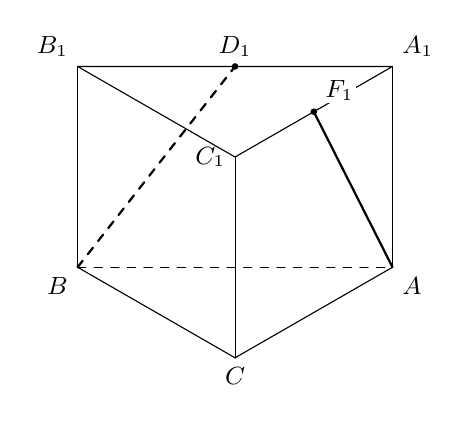
\begin{tikzpicture}[x=1cm,y=1cm,font=\small,line cap=round,line join=round]
  \coordinate (B) at (-2,0);
  \coordinate (A) at (2,0);
  \coordinate (C) at (0,-1.15);
  \coordinate (B1) at (-2,2.55);
  \coordinate (A1) at (2,2.55);
  \coordinate (C1) at (0,1.4);
  \coordinate (D1) at (0,2.55);
  \coordinate (F1) at (1,1.975);

  % Bottom triangle: the rear edge is hidden in the source projection.
  \draw[dashed] (B)--(A);
  \draw (B)--(C)--(A);
  % Top triangle and lateral edges of the right prism.
  \draw (B1)--(A1)--(C1)--cycle;
  \draw (B)--(B1) (A)--(A1) (C)--(C1);
  % The requested segments BD_1 and AF_1.
  \draw[dashed,thick] (B)--(D1);
  \draw[thick] (A)--(F1);

  \fill (D1) circle (1.2pt) (F1) circle (1.2pt);
  \node[above left] at (B1) {$B_1$};
  \node[above right] at (A1) {$A_1$};
  \node[left] at (C1) {$C_1$};
  \node[above] at (D1) {$D_1$};
  \node[fill=white,inner sep=1pt,above right=3pt] at (F1) {$F_1$};
  \node[below left] at (B) {$B$};
  \node[below right] at (A) {$A$};
  \node[below] at (C) {$C$};
\end{tikzpicture}
\end{center}
\nopagebreak[4]
（A）$\dfrac{\sqrt{30}}{10}$　　（B）$\dfrac12$　　（C）$\dfrac{\sqrt{30}}{15}$　　（D）$\dfrac{\sqrt{15}}{10}$

\Needspace{4\baselineskip}
\textbf{解析}

\Needspace{5\baselineskip}
设 $BC=CA=CC_1=1$。以 $C$ 为原点，$CA$、$CB$、$CC_1$ 为 $x,y,z$ 轴（$\angle BCA=90^\circ$）：
\nopagebreak[4]
\[C(0,0,0),\ A(1,0,0),\ B(0,1,0),\ A_1(1,0,1),\ B_1(0,1,1),\ C_1(0,0,1).\]
\Needspace{5\baselineskip}
$D_1$ 为 $A_1B_1$ 中点 $\Rightarrow D_1\left(\tfrac12,\tfrac12,1\right)$；$F_1$ 为 $A_1C_1$ 中点 $\Rightarrow F_1\left(\tfrac12,0,1\right)$。
\nopagebreak[4]
\[\overrightarrow{BD_1}=\left(\tfrac12,-\tfrac12,1\right),\quad |\overrightarrow{BD_1}|=\sqrt{\tfrac14+\tfrac14+1}=\frac{\sqrt6}{2};\]
\nopagebreak[4]
\[\overrightarrow{AF_1}=\left(-\tfrac12,0,1\right),\quad |\overrightarrow{AF_1}|=\sqrt{\tfrac14+1}=\frac{\sqrt5}{2};\]
\nopagebreak[4]
\[\overrightarrow{BD_1}\cdot\overrightarrow{AF_1}=-\tfrac14+0+1=\frac34.\]
两直线所成角取锐角：$\cos\alpha=\dfrac{3/4}{(\sqrt6/2)(\sqrt5/2)}=\dfrac{3/4}{\sqrt{30}/4}=\dfrac{3}{\sqrt{30}}=\dfrac{\sqrt{30}}{10}$。

\textbf{验算：} 数值 $\dfrac{3}{\sqrt{30}}\approx0.5477$，与 $\dfrac{\sqrt{30}}{10}\approx0.5477$ 一致 （成立）。合理性：$\overrightarrow{BD_1}$ 与 $\overrightarrow{AF_1}$ 的夹角约为 $56.8^\circ$，介于 $0^\circ$ 与 $90^\circ$，符合两异面直线夹角的取值范围 （成立）。

\gkanswer{答案：A。}

\par\medskip

\end{answer}
\begin{answer}
\gksolhead{16}{}

\textbf{题目}：

\Needspace{5\baselineskip}
不等式
\nopagebreak[4]
\[
\left(\dfrac13\right)^{x^2-8}>3^{-2x}
\]
的解集是\underline{\qquad\qquad}。

\Needspace{4\baselineskip}
\textbf{解析}

\Needspace{5\baselineskip}
$\left(\dfrac13\right)^{x^2-8}=3^{-(x^2-8)}=3^{8-x^2}$。底数 $3>1$，指数函数递增，故原不等式等价于
\nopagebreak[4]
\[8-x^2>-2x\iff x^2-2x-8<0\iff (x-4)(x+2)<0\iff -2<x<4.\]

\textbf{验算：} $x=0,3$ 满足严格不等号；$x=-2,4$ 为边界、不满足；$x=5$ 不在解集内。

\gkanswer{答案：$(-2,\,4)$。}

\par\medskip

\end{answer}
\begin{answer}
\gksolhead{17}{}

\textbf{题目}：

已知圆台上、下底面圆周都在球面上，且下底面过球心，母线与底面所成的角为 $\dfrac\pi3$，则圆台的体积与球体积之比为\underline{\qquad\qquad}。

\Needspace{4\baselineskip}
\textbf{解析}

设球半径 $R$。下底面圆周在球面上且下底面过球心，故下底面是大圆，半径 $r_2=R$，其所在平面过球心。圆台为直圆台，上下底面圆心都在垂直于底面的公共轴上，该轴过球心。设上底面圆所在平面与球心距离为 $h$，则圆台高为 $h$，上底半径 $r_1=\sqrt{R^2-h^2}$。

\Needspace{5\baselineskip}
母线与底面所成角为 $\dfrac{\pi}{3}$，在轴截面内母线的水平投影长为 $R-r_1$、竖直投影长为 $h$，故
\nopagebreak[4]
\[\tan\frac{\pi}{3}=\frac{h}{R-r_1}\ \Longrightarrow\ h=\sqrt3\,(R-r_1).\]
\Needspace{5\baselineskip}
又 $h^2+r_1^2=R^2$，代入：
\nopagebreak[4]
\[3(R-r_1)^2+r_1^2=R^2\ \Longrightarrow\ 4r_1^2-6Rr_1+2R^2=0\ \Longrightarrow\ (2r_1-R)(r_1-R)=0.\]
\Needspace{5\baselineskip}
$r_1=R$ 给出 $h=0$（退化为圆柱），舍去；故 $r_1=\dfrac{R}{2}$，$h=\dfrac{\sqrt3}{2}R$。

\nopagebreak[4]
\[V_{\text{\text{台}}}=\frac{\pi h}{3}\left(r_1^2+r_1R+R^2\right)=\frac{\pi}{3}\cdot\frac{\sqrt3 R}{2}\cdot\frac{7R^2}{4}=\frac{7\sqrt3\,\pi R^3}{24},\qquad V_{\text{\text{球}}}=\frac{4\pi R^3}{3}.\]
\nopagebreak[4]
\[\frac{V_{\text{\text{台}}}}{V_{\text{\text{球}}}}=\frac{7\sqrt3}{24}\cdot\frac{3}{4}=\frac{7\sqrt3}{32}.\]

\textbf{验算（取 $R=2$）：} $r_1=1$，$h=\sqrt3$，母线长 $\sqrt{h^2+(R-r_1)^2}=\sqrt{3+1}=2$，与底面夹角 $\arctan\dfrac{\sqrt3}{1}=60^\circ$ （成立）。$V_{\text{\text{台}}}=4.041\pi$，$V_{\text{\text{球}}}=\dfrac{32\pi}{3}=10.667\pi$，比值 $0.3789=\dfrac{7\sqrt3}{32}$ （成立）。

\textbf{源疑点（说明性）：} “下底面过球心”若读作“下底面\textbf{圆周}过球心”，则下底圆半径与所在平面到球心的距离同为 $s=\dfrac{R}{\sqrt2}$。此时同侧情形由 $h=\sqrt3(r_2-r_1)$ 与 $r_1^2=R^2-(s+h)^2$ 联立得 $h<0$，无正解；异侧情形得 $r_1<0$，不合。故只能取“下底面\textbf{所在平面}过球心”（大圆）一解，答案唯一。建议上游对原页措辞确认。

\gkanswer{答案：$\frac{7\sqrt3}{32}$。}

\par\medskip

\end{answer}
\begin{answer}
\gksolhead{18}{}

\textbf{题目}：

函数 $y=\sin\left(x-\dfrac\pi6\right)\cos x$ 的最小值是\underline{\qquad\qquad}。

\Needspace{4\baselineskip}
\textbf{解析}

\nopagebreak[4]
\[y=\sin\left(x-\frac{\pi}{6}\right)\cos x=\frac12\left[\sin\left(2x-\frac{\pi}{6}\right)+\sin\left(-\frac{\pi}{6}\right)\right]=\frac12\sin\left(2x-\frac{\pi}{6}\right)-\frac14.\]
$\sin\left(2x-\dfrac{\pi}{6}\right)$ 的最小值为 $-1$，故 $y_{\min}=-\dfrac12-\dfrac14=-\dfrac34$。

\textbf{验算：} 取 $2x-\dfrac{\pi}{6}=-\dfrac{\pi}{2}$，即 $x=-\dfrac{\pi}{6}$：$y=\sin\left(-\dfrac{\pi}{3}\right)\cos\left(-\dfrac{\pi}{6}\right)=\left(-\dfrac{\sqrt3}{2}\right)\cdot\dfrac{\sqrt3}{2}=-\dfrac34$ （成立），取到最小值。

\gkanswer{答案：$-\frac34$。}

\par\medskip

\end{answer}
\begin{answer}
\gksolhead{19}{}

\textbf{题目}：

直线 $l$ 过抛物线 $y^2=a(x+1)\quad(a>0)$ 的焦点，并且与 $x$ 轴垂直，若 $l$ 被抛物线截得的线段长为 $4$，则 $a=$\underline{\qquad\qquad}。

\Needspace{4\baselineskip}
\textbf{解析}

抛物线 $y^2=a(x+1)$ 的顶点为 $(-1,0)$，开口向右，$4p=a$，焦点为 $\left(-1+\dfrac a4,\,0\right)$。过焦点且垂直于 $x$ 轴的直线 $l:\ x=-1+\dfrac a4$ 与抛物线交于 $y^2=a\cdot\dfrac a4=\dfrac{a^2}{4}$，即 $y=\pm\dfrac a2$，截得线段长 $=a$。由 $a=4$。

\textbf{验算：} $a=4$ 时 $y^2=4(x+1)$，焦点 $\left(-1+1,0\right)=(0,0)$ 即原点，$l$ 为 $y$ 轴，与抛物线交于 $(0,\pm2)$，弦长 $4$ （成立）。

\gkanswer{答案：$a=4$。}

\par\medskip

\end{answer}
\begin{answer}
\gksolhead{20}{}

\textbf{题目}：

四个不同的小球放入编号为 $1,2,3,4$ 的四个盒中，则恰有一个空盒的放法共有\underline{\qquad\qquad}种（用数字作答）。

\Needspace{4\baselineskip}
\textbf{解析}

恰有一个空盒，即 $4$ 个球进入 $3$ 个盒且每盒非空。

第一步：选定空盒，$4$ 种。
\Needspace{5\baselineskip}
第二步：$4$ 个不同球放入剩下的 $3$ 个不同盒，每盒至少一球。用容斥：
\nopagebreak[4]
\[3^4-\mathrm C_3^1\cdot2^4+\mathrm C_3^2\cdot1^4=81-48+3=36.\]
合计 $4\times36=144$。

\textbf{验算（按分配型另算）：} 非空分配到 $3$ 盒只能是 $2+1+1$ 型：选装 $2$ 球的盒 $3$ 种，选该盒中的两球 $\mathrm C_4^2=6$ 种，余下两球分入余下两盒 $2!=2$ 种，得 $3\times6\times2=36$ （成立），与容斥结果一致。总数为 $4\times36=144$。

\gkanswer{答案：$144$ 种。}

\par\medskip

\end{answer}
\begin{answer}
\gksolhead{21}{}

\textbf{题目}：

在复平面上，一个正方形的四个顶点按照逆时针方向依次为 $Z_1,Z_2,Z_3,O$（其中 $O$ 是原点），已知 $Z_2$ 对应复数 $Z_2=1+\sqrt3i$。求 $Z_1$ 和 $Z_3$ 对应的复数。

\Needspace{4\baselineskip}
\textbf{解析}

正方形的顶点按逆时针依次为 $Z_1,Z_2,Z_3,O$，故 $O$ 与 $Z_2$ 是对角顶点，$Z_1$ 与 $Z_3$ 是另一条对角的端点。

\Needspace{5\baselineskip}
方法一（旋转）：以 $O\to Z_1$ 为边、逆时针转 $90^\circ$ 得 $Z_1\to Z_2$，故
\nopagebreak[4]
\[Z_2=Z_1+iZ_1=(1+i)Z_1\ \Longrightarrow\ Z_1=\frac{Z_2}{1+i}=\frac{(1+\sqrt3 i)(1-i)}{2}=\frac{1+\sqrt3}{2}+\frac{\sqrt3-1}{2}i.\]
又 $Z_3=O+iZ_1=iZ_1=\dfrac{1-\sqrt3}{2}+\dfrac{1+\sqrt3}{2}i$。

方法二（对角线）：$OZ_2$ 的中点 $M=\dfrac{1+\sqrt3 i}{2}$，另一条对角线 $Z_1Z_3$ 与 $OZ_2$ 垂直、等长、同中点，故 $Z_{1,3}=M\pm\dfrac12 i(1+\sqrt3 i)$，即 $M\mp\dfrac{\sqrt3-i}{2}$，与上面的结果一致；按逆时针顺序确定 $Z_1$ 取“顺时针一侧”，$Z_3$ 取另一侧。

\textbf{验算：} $Z_2=(1+i)Z_1$：$(1+i)\left(\frac{1+\sqrt3}{2}+\frac{\sqrt3-1}{2}i\right)=\frac{(1+\sqrt3)-(\sqrt3-1)}{2}+\frac{(1+\sqrt3)+(\sqrt3-1)}{2}i=1+\sqrt3 i$ （成立）。几何核验：$|Z_1|=|Z_3|=\sqrt2$，$|Z_2|=2$，$|Z_1-Z_3|=|1.732-i|=2$，两对角线等长且垂直 （成立）；四点 $O(0,0)$、$Z_1(1.366,0.366)$、$Z_2(1,1.732)$、$Z_3(-0.366,1.366)$ 依 $O\to Z_1\to Z_2\to Z_3$ 的叉积为正，确为逆时针 （成立）。

\gkanswer{答案：$Z_1=\dfrac{1+\sqrt3}{2}+\dfrac{\sqrt3-1}{2}i$，$Z_3=\dfrac{1-\sqrt3}{2}+\dfrac{1+\sqrt3}{2}i$。}

\par\medskip

\end{answer}
\begin{answer}
\gksolhead{22}{}

\textbf{题目}：

求 $\sin^2 20^\circ+\cos^2 50^\circ+\sin20^\circ\cos50^\circ$ 的值。

\Needspace{4\baselineskip}
\textbf{解析}

记 $A=20^\circ$。由 $\cos50^\circ=\cos(90^\circ-40^\circ)=\sin40^\circ$，原式 $=\sin^2 20^\circ+\sin^2 40^\circ+\sin20^\circ\sin40^\circ$。

\Needspace{5\baselineskip}
用降幂与积化和差：
\nopagebreak[4]
\[\sin^2 20^\circ=\frac{1-\cos40^\circ}{2},\quad \sin^2 40^\circ=\frac{1-\cos80^\circ}{2},\quad \sin20^\circ\sin40^\circ=\frac{\cos20^\circ-\cos60^\circ}{2}.\]
\Needspace{5\baselineskip}
三式相加：
\nopagebreak[4]
\[1-\frac{\cos40^\circ+\cos80^\circ}{2}+\frac{\cos20^\circ}{2}-\frac14=\frac34-\frac{2\cos60^\circ\cos20^\circ}{2}+\frac{\cos20^\circ}{2}=\frac34-\frac{\cos20^\circ}{2}+\frac{\cos20^\circ}{2}=\frac34.\]

\textbf{验算（数值）：} $\sin^2 20^\circ=0.11698$，$\cos^2 50^\circ=0.41318$，$\sin20^\circ\cos50^\circ=0.21985$，和 $=0.75001\approx\dfrac34$ （成立）。

\gkanswer{答案：$\dfrac34$。}

\par\medskip

\end{answer}
\begin{answer}
\gksolhead{23}{}

\textbf{题目}：

如图，圆柱的轴截面 $ABCD$ 是正方形，点 $E$ 在底面的圆周上，$AF\perp DE$，$F$ 是垂足。
\nopagebreak[4]
\begin{center}% 固定来源PDF印刷页51第23题圆柱、轴截面和垂足的示意重绘。
% 图中比例仅作示意，不添加题干未给出的度量条件。
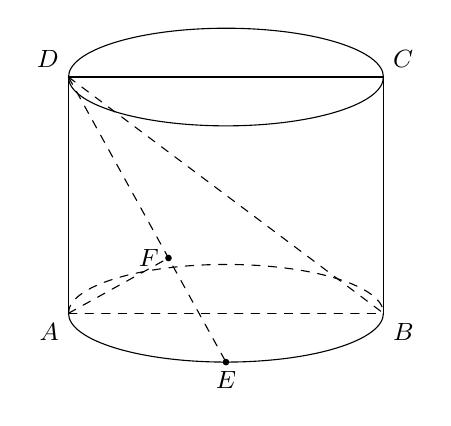
\begin{tikzpicture}[x=1cm,y=1cm,font=\small,line cap=round,line join=round]
  \coordinate (A) at (0,0);
  \coordinate (B) at (4,0);
  \coordinate (C) at (4,3);
  \coordinate (D) at (0,3);
  \coordinate (E) at (2,-.62);
  % F is the orthogonal projection of A onto DE in this schematic.
  \coordinate (F) at (1.269849,.701574);

  % Cylinder surface and circular rims; back half of the lower rim is hidden.
  \draw (D)--(A) (C)--(B);
  \draw (D)--(C);
  \draw (2,3) ellipse (2 and .62);
  \draw[dashed] (A) arc[start angle=180,end angle=0,x radius=2,y radius=.62];
  \draw (A) arc[start angle=180,end angle=360,x radius=2,y radius=.62];
  % Axial-section diagonal, DE and its perpendicular AF.
  \draw[dashed] (D)--(B);
  \draw[dashed] (A)--(B);
  \draw[dashed] (D)--(E) (A)--(F);
  \fill (E) circle (1.2pt) (F) circle (1.2pt);

  \node[above left] at (D) {$D$};
  \node[above right] at (C) {$C$};
  \node[below left] at (A) {$A$};
  \node[below right] at (B) {$B$};
  \node[below] at (E) {$E$};
  \node[left] at (F) {$F$};
\end{tikzpicture}
\end{center}
\nopagebreak[4]
（1）求证：$AF\perp DB$；

（2）如果圆柱与三棱锥 $D-ABE$ 的体积的比等于 $3\pi$，求直线 $DE$ 与平面 $ABCD$ 所成的角。

\Needspace{4\baselineskip}
\textbf{解析}

设圆柱底面半径为 $r$。轴截面 $ABCD$ 为正方形，故 $AB$ 为下底直径、$DC$ 为上底直径、$AD\parallel BC$ 为母线，边长 $AB=AD=2r$。

（1） $AB$ 是下底圆的直径且 $E$ 在下底圆上，由直径所对圆周角为直角得 $BE\perp AE$。
$DA$ 是圆柱母线，垂直于底面，故 $DA\perp BE$。
于是 $BE$ 垂直于平面 $DAE$ 内的两条相交直线 $AE$、$DA$，即 $BE\perp$ 平面 $DAE$；而 $AF\subset$ 平面 $DAE$，故 $BE\perp AF$。
又已知 $AF\perp DE$，且 $BE\cap DE=E$，所以 $AF\perp$ 平面 $BDE$。因 $DB\subset$ 平面 $BDE$，得 $AF\perp DB$。

（2） 圆柱体积 $V=\pi r^2\cdot 2r=2\pi r^3$。
\Needspace{5\baselineskip}
三棱锥 $D-ABE$ 以 $\triangle ABE$ 为底（在底面内）、以 $DA=2r$ 为高。设 $d$ 为 $E$ 到底面直径 $AB$ 的距离，则 $S_{\triangle ABE}=\dfrac12\cdot 2r\cdot d=rd$，
\nopagebreak[4]
\[V_{D-ABE}=\frac13\cdot 2r\cdot rd=\frac23r^2d.\]
由 $\dfrac{V}{V_{D-ABE}}=3\pi$ 得 $\dfrac{2\pi r^3}{\frac23 r^2 d}=3\pi$，即 $\dfrac{3\pi r}{d}=3\pi$，故 $d=r$。

$E$ 在半径为 $r$ 的圆上，到直径 $AB$ 的距离最大值为 $r$，取到时 $OE\perp AB$（$O$ 为下底圆心），且 $E$ 在平面 $ABCD$ 上的射影正是 $O$。
\Needspace{5\baselineskip}
在直角三角形 $DOE$ 中，$OE\perp$ 平面 $ABCD$，故 $\angle DOE=90^\circ$，$DO=\sqrt{DA^2+AO^2}=\sqrt{4r^2+r^2}=\sqrt5\,r$，$OE=r$。$DE$ 与平面 $ABCD$ 所成角即 $\angle ODE$：
\nopagebreak[4]
\[\tan\angle ODE=\frac{OE}{DO}=\frac{r}{\sqrt5 r}=\frac{\sqrt5}{5}.\]

\textbf{验算：} 取 $r=1$，坐标 $A(-1,0,0)$，$B(1,0,0)$，$D(-1,0,2)$，$E(0,1,0)$。
(i) 圆柱 $V=2\pi$，三棱锥 $V_{D-ABE}=\dfrac16\left|\det(\overrightarrow{AB},\overrightarrow{AE},\overrightarrow{AD})\right|=\dfrac16\left|\det\begin{pmatrix}2&0&0\\1&1&0\\0&0&2\end{pmatrix}\right|=\dfrac{4}{6}=\dfrac23$，比值 $2\pi/\frac23=3\pi$ （成立），与题设吻合。
(ii) 求 $A$ 到 $DE$ 的垂足：$F=D+t\overrightarrow{DE}=(-1+t,\,t,\,2-2t)$，由 $\overrightarrow{AF}\cdot\overrightarrow{DE}=0$ 得 $t=\dfrac23$，$F=\left(-\tfrac13,\tfrac23,\tfrac23\right)$，$\overrightarrow{AF}=\left(\tfrac23,\tfrac23,\tfrac23\right)$；$\overrightarrow{DB}=(2,0,-2)$，$\overrightarrow{AF}\cdot\overrightarrow{DB}=\tfrac43-\tfrac43=0$ （成立），与（1）一致。
(iii) 平面 $ABCD$ 为 $y=0$，$\overrightarrow{DE}=(1,1,-2)$，$\sin\alpha=\dfrac{1}{\sqrt{1+1+4}}=\dfrac{1}{\sqrt6}$，$\alpha=\arcsin\dfrac{\sqrt6}{6}=\arctan\dfrac{\sqrt5}{5}\approx24.1^\circ$ （成立）。

\gkanswer{答案：（1）见证明；（2）$\arctan\dfrac{\sqrt5}{5}$（约 $24.1^\circ$）。}

\par\medskip

\end{answer}
\begin{answer}
\gksolhead{24}{}

\textbf{题目}：

\Needspace{5\baselineskip}
某地为促进淡水鱼养殖业的发展，将价格控制在适当范围内，决定对淡水鱼养殖提供政府补贴。设淡水鱼的市场价格为 $x$ 元/千克，政府补贴为 $t$ 元/千克。根据市场调查，当 $8\le x\le14$ 时，淡水鱼的市场日供应量 $P$ 千克与市场日需求量 $Q$ 千克近似满足关系：
\nopagebreak[4]
\[
P=1000(x+t-8)\quad(x\ge8,\ t\ge0),\qquad
Q=500\sqrt{40-(x-8)^2}\quad(8\le x\le14)
\]
当 $P=Q$ 时市场价格称为市场平衡价格。

（1）将市场平衡价格表示为政府补贴的函数，并求出函数的定义域；

（2）为使市场平衡价格不高于每千克 10 元，政府补贴至少为每千克多少元？

\Needspace{4\baselineskip}
\textbf{解析}

\Needspace{5\baselineskip}
（1） 令平衡，$P=Q$：
\nopagebreak[4]
\[1000(x+t-8)=500\sqrt{40-(x-8)^2}\ \Longrightarrow\ 2(x+t-8)=\sqrt{40-(x-8)^2}.\]
\Needspace{5\baselineskip}
记 $u=x-8\in[0,6]$（因 $8\le x\le14$），则 $2(u+t)=\sqrt{40-u^2}$，两边平方整理：
\nopagebreak[4]
\[4(u+t)^2=40-u^2\ \Longrightarrow\ 5u^2+8tu+4t^2-40=0.\]
\Needspace{5\baselineskip}
解出
\nopagebreak[4]
\[u=\frac{-8t\pm\sqrt{64t^2-20(4t^2-40)}}{10}=\frac{-8t\pm4\sqrt{50-t^2}}{10}=\frac{-4t\pm2\sqrt{50-t^2}}{5}.\]
\Needspace{5\baselineskip}
因 $t\ge0$，取负号时 $u<0$，不合 $u\ge0$；故
\nopagebreak[4]
\[u=\frac{2\sqrt{50-t^2}-4t}{5},\qquad x=8+\frac{2\sqrt{50-t^2}-4t}{5}.\]
定义域由 $u\ge0$ 决定：$\sqrt{50-t^2}\ge2t\iff 50-t^2\ge4t^2\iff t^2\le10$，即 $0\le t\le\sqrt{10}$（此时 $x\le8+\frac{2\sqrt{50}}{5}\approx10.83\le14$，满足题设 $x$ 的范围）。

\Needspace{5\baselineskip}
（2） $x(t)$ 在 $[0,\sqrt{10}]$ 上严格递减（$t$ 增大时分子 $2\sqrt{50-t^2}-4t$ 严格减小）。故
\nopagebreak[4]
\[x(t)\le10\iff 8+\frac{2\sqrt{50-t^2}-4t}{5}\le10\iff 2\sqrt{50-t^2}-4t\le10\iff \sqrt{50-t^2}\le 5+2t.\]
两边非负，平方得 $50-t^2\le25+20t+4t^2$，即 $5t^2+20t-25\ge0$，$(t+5)(t-1)\ge0$，$t\ge1$。
政府补贴至少为每千克 $1$ 元。

\textbf{验算：} $t=0$：$u=\dfrac{2\sqrt{50}}{5}=2\sqrt2$，$x\approx10.83$，检查 $2u=5.657=\sqrt{40-8}$ （成立）。$t=1$：$u=\dfrac{2\sqrt{49}-4}{5}=2$，$x=10$，此时 $P=1000(10+1-8)=3000$，$Q=500\sqrt{40-4}=500\cdot6=3000$ （成立），恰好达到“不高于 10 元”的边界。$t=\sqrt{10}$：$u=\dfrac{2\sqrt{40}-4\sqrt{10}}{5}=0$，$x=8$，$P=1000\sqrt{10}$，$Q=500\sqrt{40}=1000\sqrt{10}$ （成立）。

\gkanswer{答案：（1）$x=8+\dfrac{2\sqrt{50-t^2}-4t}{5}$，$t\in[0,\sqrt{10}]$；（2）政府补贴至少为每千克 $1$ 元。}

\par\medskip

\end{answer}
\begin{answer}
\gksolhead{25}{}

\textbf{题目}：

设 $\{a_n\}$ 是由正数组成的等比数列，$S_n$ 是其前 $n$ 项和。

\Needspace{5\baselineskip}
（1）证明：
\nopagebreak[4]
\[
\frac{\lg S_n+\lg S_{n+2}}{2}<\lg S_{n+1};
\]

\Needspace{5\baselineskip}
（2）是否存在常数 $c>0$，使得
\nopagebreak[4]
\[
\frac{\lg(S_n-c)+\lg(S_{n+2}-c)}{2}=\lg(S_{n+1}-c)
\]
成立？并证明你的结论。

\Needspace{4\baselineskip}
\textbf{解析}

设 $a_n=a_1q^{n-1}$（$a_1>0,\ q>0$），$S_{k+1}=a_1+qS_k$，且 $a_{n+1}=S_{n+1}-S_n>0$。

\Needspace{5\baselineskip}
（1） 计算
\nopagebreak[4]
\[S_{n+1}^2-S_nS_{n+2}=S_{n+1}^2-S_n\left(a_1+qS_{n+1}\right)=S_{n+1}\left(S_{n+1}-qS_n\right)-a_1S_n.\]

\nopagebreak[4]
\[=a_1S_{n+1}-a_1S_n=a_1a_{n+1}>0.\]
\Needspace{5\baselineskip}
故 $S_nS_{n+2}<S_{n+1}^2$。又 $S_n>0$，$S_{n+2}>0$，$S_{n+1}>0$，由 $\lg$ 的单调性，
\nopagebreak[4]
\[\lg S_n+\lg S_{n+2}<2\lg S_{n+1}\iff \frac{\lg S_n+\lg S_{n+2}}{2}<\lg S_{n+1}.\]

\Needspace{5\baselineskip}
（2） 假设存在 $c>0$ 使
\nopagebreak[4]
\[\frac{\lg(S_n-c)+\lg(S_{n+2}-c)}{2}=\lg(S_{n+1}-c)\]
\Needspace{5\baselineskip}
对一切 $n\in\mathbb N^*$ 成立，则须 $S_n-c>0$，且等价于
\nopagebreak[4]
\[(S_n-c)(S_{n+2}-c)=(S_{n+1}-c)^2.\]
\Needspace{5\baselineskip}
展开整理（$c^2$ 相消）：
\nopagebreak[4]
\[S_nS_{n+2}-S_{n+1}^2=c\left(S_n+S_{n+2}-2S_{n+1}\right).\]
左边 $=-a_1a_{n+1}$（由（1））。右边括号 $=(S_{n+2}-S_{n+1})-(S_{n+1}-S_n)=a_{n+2}-a_{n+1}=a_{n+1}(q-1)$。
\Needspace{5\baselineskip}
故
\nopagebreak[4]
\[-a_1a_{n+1}=c\,a_{n+1}(q-1)\ \Longrightarrow\ c(1-q)=a_1>0.\]
\Needspace{5\baselineskip}
由此 $q<1$ 且 $c=\dfrac{a_1}{1-q}$。但当 $0<q<1$ 时
\nopagebreak[4]
\[S_n=\frac{a_1(1-q^n)}{1-q}<\frac{a_1}{1-q}=c,\]
即 $S_n-c<0$，$\lg(S_n-c)$ 无意义，矛盾。

（$q=1$ 时右边括号为 $0$ 而左边为 $-a_1^2\ne0$，同样矛盾。）
所以不存在满足条件的常数 $c>0$。

\textbf{验算：} （i）取 $a_1=1,\ q=2$，$n=1$：$S_1S_3=1\times7=7<S_2^2=9$ （成立）；（1）的恒等式给 $a_1a_2=2=9-7$ （成立）。
（ii）把（2）的代数结论代入自检：$c=\dfrac{a_1}{1-q}$，若 $q=2$ 则 $c=-1<0$，不合 $c>0$；若 $q=\frac12$ 则 $c=2$，而 $S_1=1<2$ 使 $\lg(S_1-2)$ 无意义——两条出路都被封死，结论“不存在”稳健。

\gkanswer{答案：（1）见证明；（2）不存在这样的常数 $c>0$。}

\par\medskip

\end{answer}
\begin{answer}
\gksolhead{26}{}

\textbf{题目}：

已知椭圆 $\dfrac{x^2}{24}+\dfrac{y^2}{16}=1$，直线 $l$：$\dfrac{x}{12}+\dfrac{y}{8}=1$
\Needspace{5\baselineskip}
$P$ 是 $l$ 上一点，射线 $OP$ 交椭圆于点 $R$，又点 $Q$ 在 $OP$ 上且满足
\nopagebreak[4]
\[
|OQ|\cdot|OP|=|OR|^2
\]
当点 $P$ 在 $l$ 上移动时，求点 $Q$ 的轨迹方程，并说明轨迹是什么曲线。

\Needspace{4\baselineskip}
\textbf{解析}

设 $Q(x,y)$（$Q\ne O$）。因 $Q$ 在射线 $OP$ 上，可设 $P=\mu Q$（$\mu>0$）；同理设 $R=\nu Q$（$\nu>0$）。

$R$ 在椭圆上：$\nu^2\left(\dfrac{x^2}{24}+\dfrac{y^2}{16}\right)=1$，故 $\nu=\dfrac{1}{\sqrt{x^2/24+y^2/16}}$，且 $|OR|=\nu|OQ|$，$|OP|=\mu|OQ|$。

条件 $|OQ|\cdot|OP|=|OR|^2$ 化为 $\mu|OQ|^2=\nu^2|OQ|^2$，即 $\mu=\nu^2=\dfrac{1}{x^2/24+y^2/16}$。

\Needspace{5\baselineskip}
$P$ 在直线 $\dfrac{x}{12}+\dfrac{y}{8}=1$（即 $2x+3y=24$）上：
\nopagebreak[4]
\[2(\mu x)+3(\mu y)=24\ \Longrightarrow\ \mu(2x+3y)=24\ \Longrightarrow\ \frac{2x+3y}{x^2/24+y^2/16}=24.\]
\Needspace{5\baselineskip}
即 $2x+3y=24\left(\dfrac{x^2}{24}+\dfrac{y^2}{16}\right)=x^2+\dfrac32y^2$，整理得
\nopagebreak[4]
\[2x^2+3y^2-4x-6y=0\iff 2(x-1)^2+3(y-1)^2=5\iff \frac{(x-1)^2}{5/2}+\frac{(y-1)^2}{5/3}=1.\]

\textbf{为何去掉原点：} 由 $\mu(2x+3y)=24$ 与 $\mu>0$ 得 $2x+3y>0$；而原点使 $\mu$ 的分母 $\dfrac{x^2}{24}+\dfrac{y^2}{16}=0$，$\nu$ 无定义，亦对应 $|OR|=0$，不可能。反之，该椭圆除原点外处处满足 $2x+3y>0$（椭圆与直线 $2x+3y=0$ 在原点相切，整体位于 $2x+3y\ge0$ 一侧），故每个这样的点 $Q$ 都唯一确定一条与 $l$ 相交的射线，进而唯一确定 $P$——轨迹恰为“椭圆去掉原点”。

\textbf{验算：}
\begin{itemize}
\item $P(12,0)$：$|OP|=12$，射线交椭圆于 $x=\sqrt{24}=2\sqrt6$，$\nu^2=\frac{24}{144}=\frac16$，$Q=(2,0)$。代入轨迹：$2(1)^2+3(1)^2=5$ （成立）。
\item $P(0,8)$：$|OP|=8$，交椭圆于 $y=4$，$\nu^2=\frac{16}{64}=\frac14$，$Q=(0,2)$。代入：$2(1)^2+3(1)^2=5$ （成立）。
\item $P(6,4)$（在 $l$ 上：$12+12=24$）：$\nu^2=\frac{1}{36/24+16/16}=\frac{1}{2.5}=0.4$，$Q=(2.4,1.6)$。代入：$2(1.4)^2+3(0.6)^2=3.92+1.08=5$ （成立）。
\item 极端情形：$P$ 沿 $l$ 趋于无穷，$\nu^2\to0$，$Q\to O$ 但不取到，与“去掉原点”一致 （成立）。
\end{itemize}

\gkanswer{答案：$2x^2+3y^2-4x-6y=0$（中心 $(1,1)$ 的椭圆），除去原点。}

\par\medskip

\end{answer}